
\appendix
\section{Proofs}
\begin{lemma}
	\label{thm:complexity}
	Solving the ER-SSAT and RE-SSAT problems are $\mathrm{NP}^{\mathrm{PP}}$ hard~\cite{littman2001stochastic}.
\end{lemma}

\begin{proof}[Proof of Lemma~\ref{thm:complexity}]
	The decision version of ER-SSAT problem is 
	\begin{equation}
		\Phi := \exists a_1,\dots, \exists a_n, \R^{p_{x_1}}x_1, \dots, \R^{p_{x_m}}x_m. \; \Pr[\phi_{\hat{y}}] \geq t,\notag
	\end{equation}
	where $t$ is a threshold in $[0,1]$.
	It is exactly the an E-MAJSAT (or threshold SAT) problem which is $NP^{PP}$ hard~\cite{littman2001stochastic}.
	If there's no random variable and $t=1$, ER-SSAT reduces to a SAT problem, which is NP-hard. If there's no existential variable, ER-SSAT reduces to a MAJSAT problem, which is PP-hard.
	Similar arguments also hold for RE-SSAT problem.
\end{proof}

\begin{equation}
\Phi_{\mathsf{UR}} := \forall \sensitive_1,\dots, \forall \sensitive_n,
\R^{p_{1}}\nonsensitive_1, \dots, \R^{p_{m}}\nonsensitive_m,   \; \phi_{\hat{Y}}.
\label{eq:ar}
\end{equation}
\begin{equation}
\Phi'_{\mathsf{ER}} := \exists \sensitive_1,\dots, \exists \sensitive_n,
\R^{p_{1}}\nonsensitive_1, \dots, \R^{p_{m}}\nonsensitive_m,   \; \neg \phi_{\hat{Y}}.
\label{eq:er_complement}
\end{equation}
\begin{lemma}\label{thm:dual}
	Given Eq.~\eqref{eq:ar} and~\eqref{eq:er_complement},	$ \Pr[\Phi_{\mathsf{UR}}] = 1 - \Pr[\Phi'_{\mathsf{ER}}]  $.
\end{lemma}

\begin{proof}[Proof of Lemma~\ref{thm:dual}]
	Both $ \Phi_{\mathsf{UR}} $ and $ \Phi'_{\mathsf{ER}} $ have  random quantified variables in the identical order in the prefix. According to the definition of SSAT formulas,
\begin{equation}
\Pr[\Phi_{\mathsf{UR}}] = \min\limits_{a_1, \dots,a_n} \Pr[\phi_{\hat{Y}}] \text{ and } \Pr[\Phi'_{\mathsf{ER}}] = \max\limits_{a_1, \dots,a_n} \Pr[\neg\phi_{\hat{Y}}].\notag
\end{equation}
We can show the following duality between ER-SSAT and UR-SSAT,
\begin{equation}
\begin{split}
\Pr[\Phi'_{\mathsf{ER}}] &= \max\limits_{a_1, \dots,a_n} \Pr[\neg\phi_{\hat{Y}}]  \\
&= \min\limits_{a_1, \dots,a_n} (1 - \Pr[\phi_{\hat{Y}}])\\
&= 1 - \min\limits_{a_1, \dots,a_n}  \Pr[\phi_{\hat{Y}}]\\
&= 1 - \Pr[\Phi_{\mathsf{UR}}].\notag
\end{split}
\end{equation}
\end{proof}


\begin{lemma}
	\label{lm:equivalence}
	Let $ \Phi_{\mathbf{a}} $ be the RE-SSAT formula for computing the PPV of the compound protected group $ \mathbf{a} \in A $. If $ \Phi_{\mathsf{ER}} $ is the ER-SSAT formula for learning the most favored group and $ \Phi_{\mathsf{UR}} $ is the UR-SSAT formula for learning the least favored group, then
	$\max_{\mathbf{a}} \; \Pr[\Phi_{\mathbf{a}}] = \Pr[\Phi_{\mathsf{ER}}]$   
	and
	$\min_{\mathbf{a}} \; \Pr[\Phi_{\mathbf{a}}] = \Pr[\Phi_{\mathsf{UR}}]$.   
\end{lemma}

\begin{proof}[Proof of Lemma~\ref{lm:equivalence}] 
	\blue{It is trivial} that the PPV of most favored group $ \mathbf{a}_{\mathsf{fav}} $ is the maximum PPV of all compound groups $ \mathbf{a} \in A $. Similarly, the PPV of the least favored group $ \mathbf{a}_{\mathsf{unfav}} $ is the minimum PPV of all compound groups $ \mathbf{a} \in A $.
	
	By construction of the SSAT formulas, the PPV of $ \mathbf{a}_{\mathsf{fav}} $ and $ \mathbf{a}_{\mathsf{unfav}} $ are $ \Pr[\Phi_{\mathsf{ER}}] $ and $ \Pr[\Phi_{\mathsf{UR}}] $ respectively. Since $ \Pr[\Phi_{\mathbf{a}}] $ is the PPV of the compound group $ \mathbf{a} $, 
	\begin{equation}
	\begin{split}
		\max_{\mathbf{a}} \; \Pr[\Phi_{\mathbf{a}}] = \Pr[\Phi_{\mathsf{ER}}]
	\text{ and }
	\min_{\mathbf{a}} \; \Pr[\Phi_{\mathbf{a}}] = \Pr[\Phi_{\mathsf{UR}}].\notag
	\end{split}
	\end{equation}
\end{proof}


\section{Practical Settings}
In this section, we  relax assumptions of Boolean classifiers and Boolean attributes and extend {\framework} to verify fairness metrics in a more practical setting. 
We first discuss the input classifiers of {\framework} in the following.

\subsubsection{Beyond CNF Classifiers.}
In the presented SSAT approach for verifying fairness, we assume the classifier $ \hat{Y} $ to be represented as a CNF formula.  In the literature of interpretable machine learning, several studies have been conducted for learning CNF classifiers in the supervised learning setting, which include but are not limited to the work of~\cite{angelino2017learning,malioutov2018mlic,ghosh19incremental,yu2020computing}.  However, {\framework} can be extended beyond CNF classifiers, in particular to decision trees and linear classifiers that are widely adopted in the ML fairness studies~\cite{zemel2013learning,zafar2017fairness,xu2019achieving,zhang2019faht,raff2018fair,friedler2019comparative}.

\textbf{Encoding Decision Trees as CNF.} Existing  rule-based classifiers, for example, binary decision trees  can be trivially encoded as  CNF formulas.  In the binary decision tree, each node in the tree is a literal. A path  from the root to the leaf is a conjunction of literals (hence, a path is a clause) and the tree itself is a disjunction of all paths (or  clauses). In order to derive a CNF representation $ \phi $ of the decision tree, we first construct a DNF by considering all paths terminating at leaves with negative class label ($ \hat{y} = 0 $) and then complement it to a CNF using De Morgan's rule. Therefore, for any input that is classified positive by the decision tree satisfies $ \phi $ and vice versa. In {\frameworklearn} for learning the least favored group, we can construct a negated CNF classifier in Eq.~\ref{eq:er_complement} by only including paths terminating on positive labeled leaves. 

\textbf{Encoding Linear Classifiers as CNF.} Linear classifiers on Boolean attributes can  be encoded into CNF formulas using pseudo-Boolean encoding~\cite{philipp2015pblib}. We consider a linear classifier  $ W\cdot X + b \ge 0 $ on Boolean attributes $ X $ with weights $ W \in \mathcal{R}^{|X}| $ and bias $ b \in \mathcal{R} $.  We first normalize $ W$ and $b $ in $ [-1,1] $ and then round to integers so that the decision boundary becomes a pseudo-Boolean constraint, e.g., \textit{at-least} $ k $ constraint.  We then apply  pseudo-Boolean constraints to CNF translation to encode the decision boundary to CNF. This encoding usually introduces additional Boolean variables and results in large CNF. In order to generate a smaller CNF, we can apply thresholding techniques on the weights $ W $ to consider attributes with higher weights only. For instance, if the weight $  |w_i| \le \lambda $ for a threshold $ \lambda $ and $ w_i \in W $, we can set $ w_i = 0 $. Thus,  lower weighted (hence less important) attributes do not appear in the encoded CNF.  Finally, to construct the negated classifier in the SSAT formula in Eq.~\ref{eq:er_complement}, we encode $ W\cdot X + b < 0 $ to CNF using \textit{at-most} $ k $ encoding. 

In practical problems, attributes are generally real-valued or categorical. We next discuss how {\framework} can work beyond Boolean attributes. 


\subsubsection{Beyond Boolean Attributes.}
Classifiers that are already represented in CNF are usually trained on a Boolean abstraction of the input attributes where  each categorical attribute is one-hot encoded  and each real-valued attribute is discretized into a set of Boolean attributes~\cite{LKCL2019,GMM20}. Thus, {\framework} can verify CNF classifiers readily. 

\textbf{Decision Trees.} In case of binary decision tree classifiers, the input attributes are numerical or categorical, but each attribute is compared against a constant in each internal node of the tree. Hence, we fix a Boolean variable for each internal node where the Boolean assignment to the variable decides one of the two branches to choose from the current node.  

\textbf{Linear Classifiers.} Linear classifiers are generally trained on numerical attributes where we apply following discretization. Consider a numerical attribute $ x $ where $ w $ is its weight. We want to discretize $ x $ to a set $ \mathbf{B} $ of Boolean attributes and recalculate the weights of the variables in $ \mathbf{B} $ from $ w $. For discretization, we simply consider interval-based approach where for each interval (or bin) in the continuous space of $ x $, we consider a Boolean variable $ b_i \in \mathbf{B} $ such that $ b_i $ is assigned $ \top $ (or $ 1 $) when the attribute-value of $ x $ lies within the interval and $ b_i $ is assigned $ \bot $ (or $ 0 $) otherwise. Let $ \mu_i $ be the mean of the interval where  $ b_i $ can be $ \top $. We then fix the revised weight of $ b_i $ to be $ \mu_i\cdot w $. We can show trivially that if we consider infinite number of intervals, $ x \approx \sum_i \mu_ib_i $. 


\begin{example}[ER-SSAT encoding]
	\label{example:er_ssat}
	Here, we illustrate the ER-SSAT encodings for learning the most favored and the least favored group in presence of multiple protected groups. As the example in Figure~\ref{fig:fair_example} is degenerate for this purpose, we introduce another protected group `sex $ \in $ \{male, female\}'. Consider a Boolean variable $ S $ for `sex' where the literal $ S $ denotes `sex = male'. With this new protected attribute, let the classifier be  $\alg \triangleq (\neg F \vee I \vee S) \wedge (F \vee J)$, where $ F,I,J $ have same distributions as discussed in Example~\ref{example:re_ssat}. 
	Hence, we obtain the ER-SSAT formula of $\alg$ to learn the most favored group:
	\begin{equation}
	\Phi_{\mathsf{ER}} :=  \exists S,\exists A, \R^{0.41}F, \R^{0.93}I, \R^{0.09}J, \; (\neg F \vee I \vee S) \wedge (F \vee J).\notag
	\end{equation}
	As we solve $ \Phi_{\mathsf{ER}} $, we learn that the assignment to the existential variables $ \sigma(S) = 1, \sigma(A) = 0$, i.e. `male individuals with age $ < 40 $' is the most favored group with PPV computed as $ \Pr[\Phi_{\mathsf{ER}}] = 0.46$. Similarly, to learn the least favored group, we negate the CNF of the classifier $\alg$ to obtain the following ER-SSAT formula:
	\begin{equation}
	\Phi_{\mathsf{ER'}} :=  \exists S, \exists A, \R^{0.41}F, \R^{0.93}I, \R^{0.09}J, \; \neg((\neg F \vee I \vee S) \wedge (F \vee J)).\notag
	\end{equation}
	Solving $ \Phi_{\mathsf{ER'}} $, we learn the assignment $ \sigma(S) = 0, \sigma(A) = 0  $ and $  \Pr[\Phi_{\mathsf{ER'}}] = 0.57 $. Thus, `female individuals with age $ < 40 $' constitute the least favored group with PPV:  $ 1-0.57 = 0.43$. 
	Thus, {\frameworklearn} allows us to learn the most and least favored groups and the corresponding discrimination.
\end{example}

\section{Experiments}
\subsection{Experimental Setup}
Since both {\framework}  and FairSquare take a  probability distribution of the attributes as input, we perform five-fold cross validation, use the train set for learning the classifier, compute distribution on the test set and finally verify fairness metrics such as disparate impact and statistical parity difference on the distribution.

\subsection{Comparative Evaluation of Two Encodings}
\iffalse
\red{Accuracy is removed}
\textbf{Accuracy.} In Section~\ref{sec:framework},  we have theoretically shown the equivalence between RE and ER encodings  and experimentally validate this in Figure~\ref{fig:equivalence} where both encodings output the same value for different fairness metrics. In the RE encoding, we consider two variations: namely `RE' and `RE(cor)' where the former does not consider the correlation between the protected and the non-protected attributes and the later includes correlation. \blue{In Figure~\ref{fig:equivalence}, we find that disparate impact usually decreases when the correlation is considered. This result is justified by the implicit dependence between the protected and non-protected attributes that the classifiers learn during training.}
\fi

%\textbf{Execution Time.} 
While both {\frameworkenum} and {\frameworklearn}  have the same output, the {\frameworklearn} encoding  improves exponentially  in runtime  than {\frameworkenum}  on both decision tree and Boolean CNF classifiers as we vary the total compound groups in Figure~\ref{fig:runtime_diff_encodings}. This analysis justifies that the na\"ive enumeration-based approach cannot verify large-scale fairness problems containing multiple protected attributes. 
\begin{figure}[t!]
	\begin{center}
		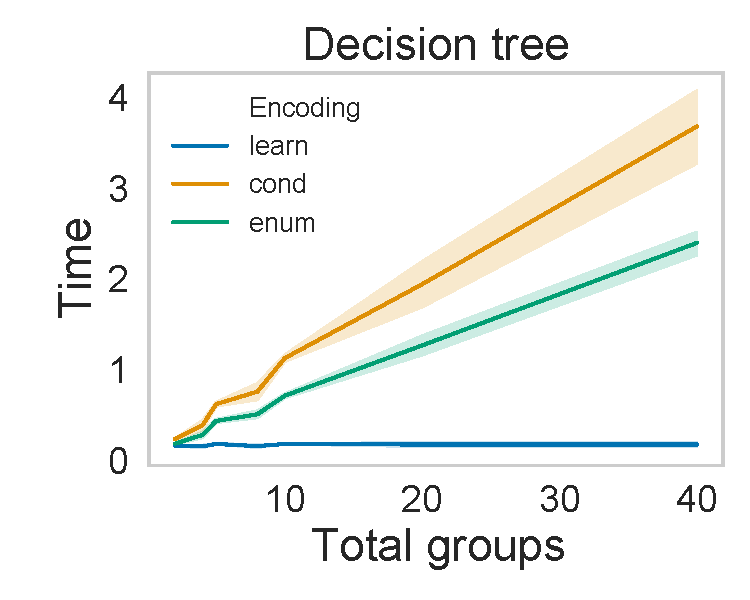
\includegraphics[scale=.32]{figures/encoding_runtime_Adult_DT.pdf}
		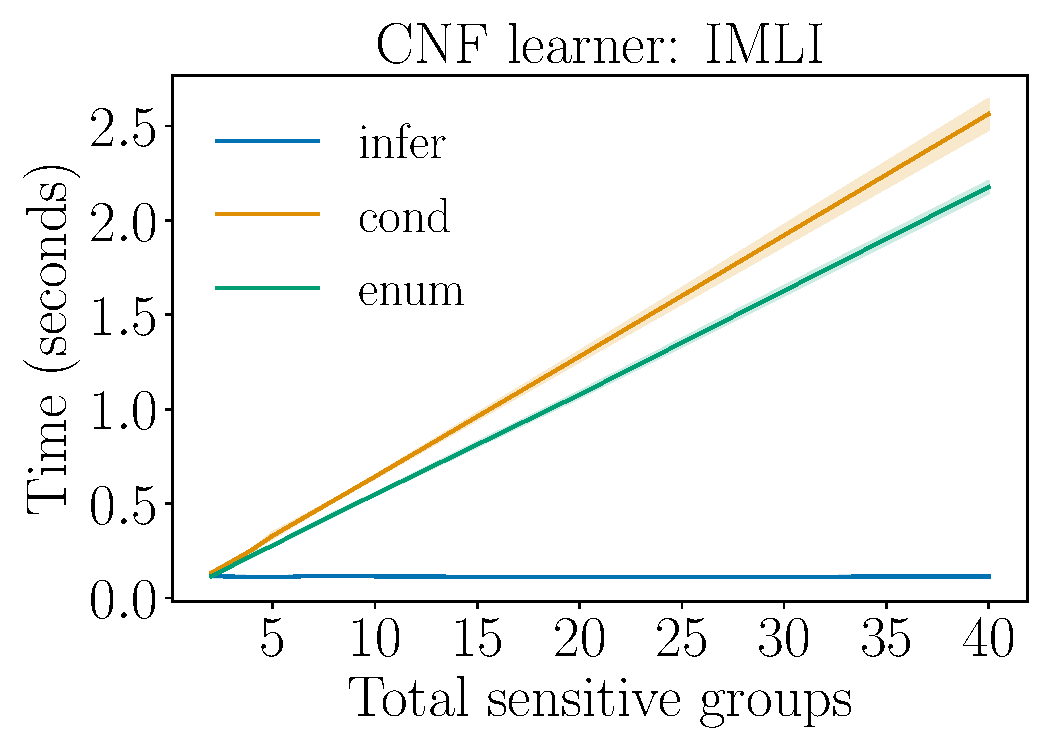
\includegraphics[scale=.32]{figures/encoding_runtime_Adult_IMLI.pdf}
		\hfill
		\caption{Runtime comparison of different encodings for varying total protected groups in the Adult dataset}
		\label{fig:runtime_diff_encodings}
	\end{center}
\end{figure}\textbf{}

\begin{table*}[t!]        
	\centering
	\caption{Verification of different fairness enhancing algorithms for multiple datasets and classifiers using {\framework}. Numbers in bold refer to fairness improvement  compared against the unprocessed (orig.) dataset. RW and OP refer to reweighing and optimized-preprocessing algorithm respectively.}\label{tab:fair_algo_verification_appendix}
	\vspace*{-.2em}
	%        \setlength{\tabcolsep}{.3em}
	\begin{tabular}{ll
			ccc
			ccc
			%            				ccc
			%            				ccc
			ccc
			ccc}
		\toprule
		\multirow{3}{*}{Classifier}& Dataset $ \rightarrow $   & 
		\multicolumn{6}{c}{German} \\
		\cmidrule(lr){3-8}
		& Protected  $ \rightarrow $ & 
                \multicolumn{3}{c}{Age}   & \multicolumn{3}{c}{Sex}  
		\\ 
		\cmidrule(lr){3-5}
		\cmidrule(lr){6-8}
		
		& Algorithm  $ \rightarrow $ &  
		orig. & RW & OP &
		orig. & RW & OP \\ 
		\midrule
		
		
		
		\multirow{3}{*}{\shortstack{Logistic \\ regression}}
		& Disparte impact&  $ 0.00 $ &  $ 0.00 $ &  $ \mathbf{0.31} $ &  $ 0.27 $ &  $ \mathbf{0.46} $ &  $ 0.17 $  \\
		& Stat. parity&  $ 0.45 $ &  $ \mathbf{0.03} $ &  $ \mathbf{0.12} $ &  $ 0.03 $ &  $ \mathbf{0.02} $ &  $ 0.07 $  \\
		& Equalized odds&  $ 0.65 $ &  $ \mathbf{0.04} $ &  $ \mathbf{0.14} $ &  $ 0.10 $ &  $ \mathbf{0.08} $ &  $ 0.13 $  \\
		\midrule
		\multirow{3}{*}{\shortstack{Decision \\ tree}}
		& Disparte impact&  $ 0.00 $ &  $ \mathbf{0.56} $ &  $ \mathbf{0.12} $ &  $ 0.35 $ &  $ \mathbf{0.37} $ &  $ \mathbf{0.38} $  \\
		& Stat. parity&  $ 0.35 $ &  $ \mathbf{0.02} $ &  $ \mathbf{0.22} $ &  $ 0.05 $ &  $ 0.10 $ &  $ 0.11 $  \\
		& Equalized odds&  $ 0.36 $ &  $ \mathbf{0.05} $ &  $ \mathbf{0.28} $ &  $ 0.06 $ &  $ 0.16 $ &  $ 0.17 $  \\
		
		
		
		
		
		
		
		
		\bottomrule
	\end{tabular}
\end{table*}


\begin{comment}
\begin{figure*}
	\begin{center}
		\subfloat{
			\includegraphics[scale=.5]{figures/DI_Adult_op_DT_race.pdf}
		}
		\subfloat{
			\includegraphics[scale=.5]{figures/SPD_Adult_op_DT_race.pdf}
		} \hfil  
		\subfloat{
			\includegraphics[scale=.5]{figures/DI_Adult_op_LR_race.pdf}
		}
		\subfloat{
			\includegraphics[scale=.5]{figures/SPD_Adult_op_LR_race.pdf}
		} \hfil  
		
		
		
		
		\subfloat{
			\includegraphics[scale=.5]{figures/DI_Adult_op_DT_sex.pdf}
		}
		\subfloat{
			\includegraphics[scale=.5]{figures/SPD_Adult_op_DT_sex.pdf}
		} \hfil
		
		\subfloat{
			\includegraphics[scale=.5]{figures/DI_Adult_op_LR_sex.pdf}
		}
		\subfloat{
			\includegraphics[scale=.5]{figures/SPD_Adult_op_LR_sex.pdf}
		} \hfil
		
	\end{center}
	
	\caption{Result for applying optimized preprocessing (op) algorithm on Adult dataset. We show results for three verifiers: RE-SSAT encoding with correlation (RE-cor), RE-SSAT encoding without correlation (RE), and statistical tool AIF360 and for two classifiers: decision tree (DT) and logistic regression (LR). If the preprocessing algorithm is successful, we observe an increase in disparate impact and a decrease in statistical parity difference as we apply the fairness algorithm. RE-cor and RE finds instances where the preprocessing algorithm fails to mitigate bias in the dataset.} 
\end{figure*}

\begin{figure*}
	\begin{center}
		
		
		\subfloat{
			\includegraphics[scale=.5]{figures/DI_German_op_DT_age.pdf}
		}
		\subfloat{
			\includegraphics[scale=.5]{figures/SPD_German_op_DT_age.pdf}
		} \hfil 
		
		\subfloat{
			\includegraphics[scale=.5]{figures/DI_German_op_LR_age.pdf}
		}
		\subfloat{
			\includegraphics[scale=.5]{figures/SPD_German_op_LR_age.pdf}
		} \hfil 
		
		
		\subfloat{
			\includegraphics[scale=.5]{figures/DI_German_op_DT_sex.pdf}
		}
		\subfloat{
			\includegraphics[scale=.5]{figures/SPD_German_op_DT_sex.pdf}
		} \hfil
		
		\subfloat{
			\includegraphics[scale=.5]{figures/DI_German_op_LR_sex.pdf}
		}
		\subfloat{
			\includegraphics[scale=.5]{figures/SPD_German_op_LR_sex.pdf}
		} \hfil
		
		
	\end{center}
	
	\caption{Result for applying optimized preprocessing (op) algorithm on German-credit dataset. We show results for three verifiers: RE-SSAT encoding with correlation (RE-cor), RE-SSAT encoding without correlation (RE), and statistical tool AIF360 and for two classifiers: decision tree (DT) and logistic regression (LR). If the preprocessing algorithm is successful, we observe an increase in disparate impact and a decrease in statistical parity difference as we apply the fairness algorithm. RE-cor and RE finds instances where the preprocessing algorithm fails to mitigate bias in the dataset.} 
\end{figure*}

\begin{figure*}
	\begin{center}
		
		
		\subfloat{
			\includegraphics[scale=.5]{figures/DI_Compas_op_DT_race.pdf}
		}
		\subfloat{
			\includegraphics[scale=.5]{figures/SPD_Compas_op_DT_race.pdf}
		} \hfil 
		
		\subfloat{
			\includegraphics[scale=.5]{figures/DI_Compas_op_LR_race.pdf}
		}
		\subfloat{
			\includegraphics[scale=.5]{figures/SPD_Compas_op_LR_race.pdf}
		} \hfil
		
		\subfloat{
			\includegraphics[scale=.5]{figures/DI_Compas_op_DT_sex.pdf}
		}
		\subfloat{
			\includegraphics[scale=.5]{figures/SPD_Compas_op_DT_sex.pdf}
		} \hfil
		
		\subfloat{
			\includegraphics[scale=.5]{figures/DI_Compas_op_LR_sex.pdf}
		}
		\subfloat{
			\includegraphics[scale=.5]{figures/SPD_Compas_op_LR_sex.pdf}
		} \hfil
		
	\end{center}
	
	\caption{Result for applying optimized preprocessing (op) algorithm on Compas dataset. We show results for three verifiers: RE-SSAT encoding with correlation (RE-cor), RE-SSAT encoding without correlation (RE), and statistical tool AIF360 and for two classifiers: decision tree (DT) and logistic regression (LR). If the preprocessing algorithm is successful, we observe an increase in disparate impact and a decrease in statistical parity difference as we apply the fairness algorithm. RE-cor and RE finds instances where the preprocessing algorithm fails to mitigate bias in the dataset.} 
\end{figure*}





\begin{figure*}
	\begin{center}
		\subfloat{
			\includegraphics[scale=.5]{figures/sampling_DI_before_Adult_op_DT_race.pdf}
		}
		\subfloat{
			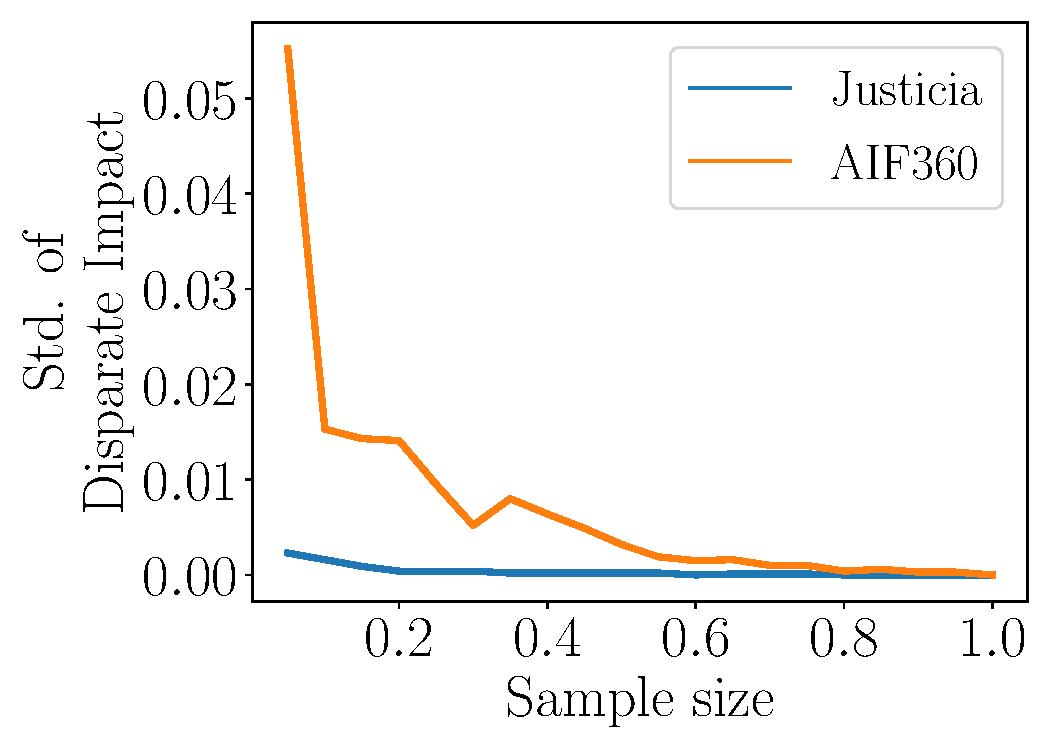
\includegraphics[scale=.5]{figures/sampling_DI_after_Adult_op_DT_race.pdf}
		} \hfil  
		\subfloat{
			\includegraphics[scale=.5]{figures/sampling_DI_before_Adult_op_LR_race.pdf}
		}
		\subfloat{
			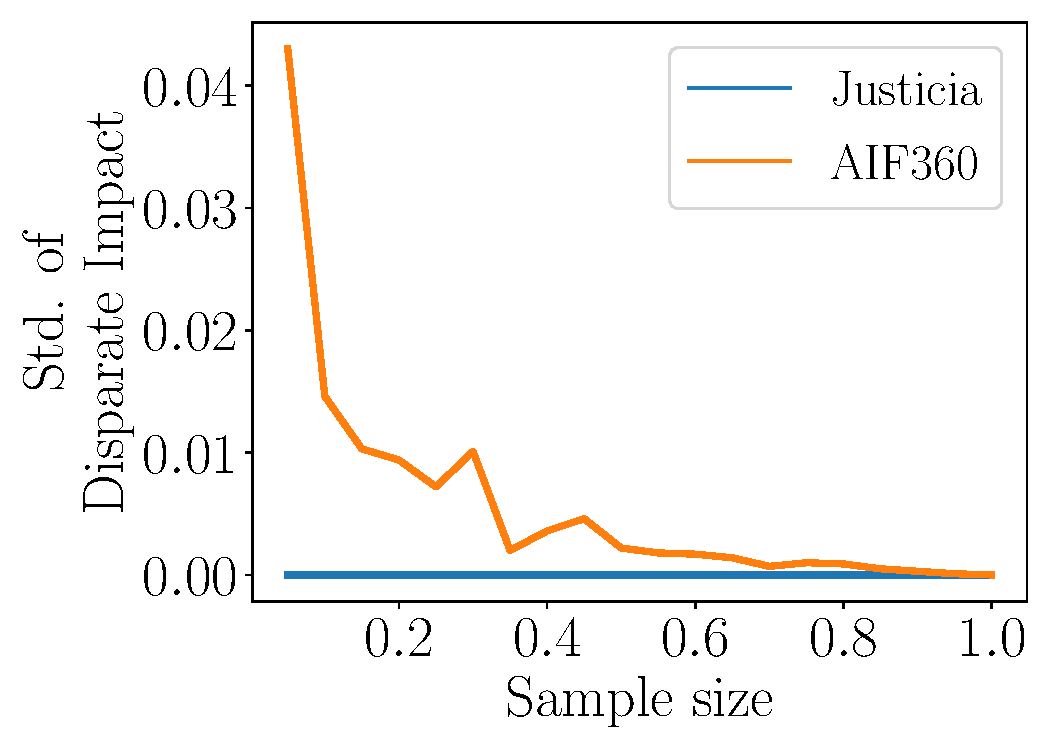
\includegraphics[scale=.5]{figures/sampling_DI_after_Adult_op_LR_race.pdf}
		} \hfil  
		
		
		
		
		\subfloat{
			\includegraphics[scale=.5]{figures/sampling_DI_before_Adult_op_DT_sex.pdf}
		}
		\subfloat{
			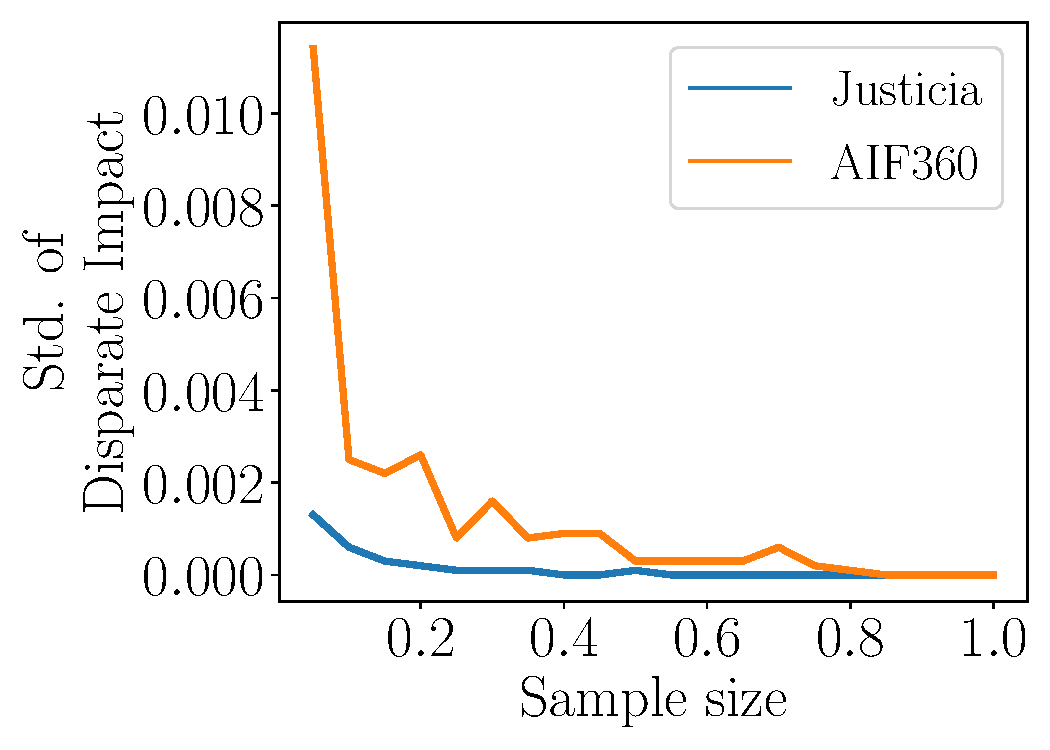
\includegraphics[scale=.5]{figures/sampling_DI_after_Adult_op_DT_sex.pdf}
		} \hfil
		
		\subfloat{
			\includegraphics[scale=.5]{figures/sampling_DI_before_Adult_op_LR_sex.pdf}
		}
		\subfloat{
			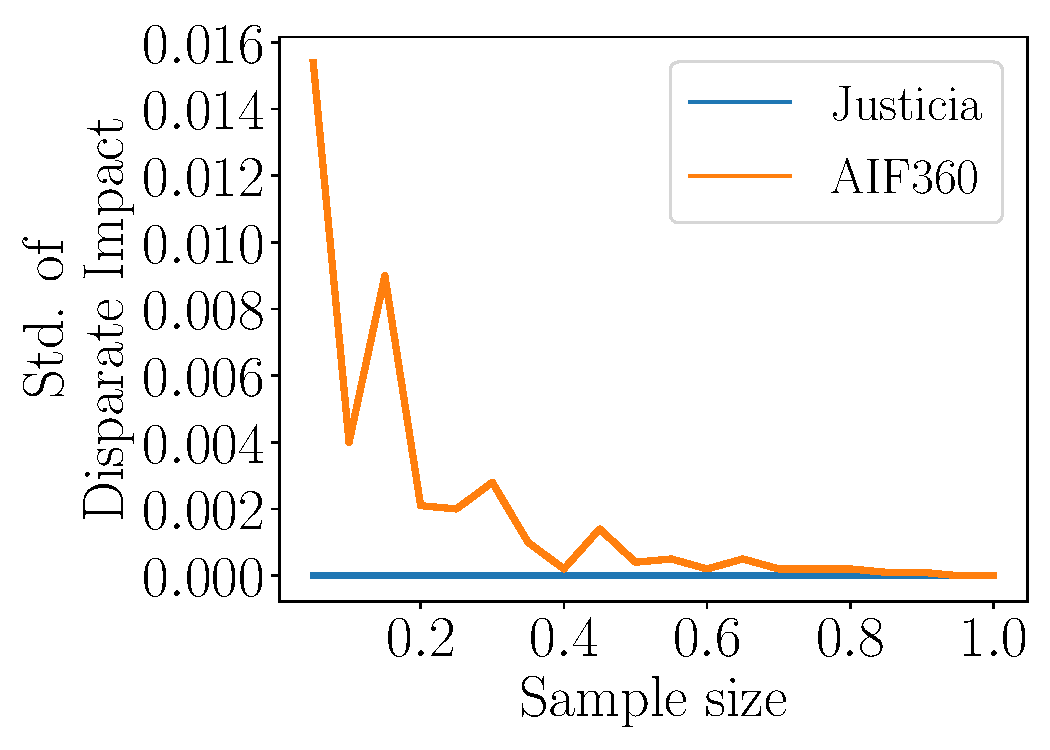
\includegraphics[scale=.5]{figures/sampling_DI_after_Adult_op_LR_sex.pdf}
		} \hfil
		
	\end{center}
	
	\caption{Effect of sampling.} 
\end{figure*}

\begin{figure*}
	\begin{center}
		\subfloat{
			\includegraphics[scale=.5]{figures/sampling_DI_before_Compas_op_DT_race.pdf}
		}
		\subfloat{
			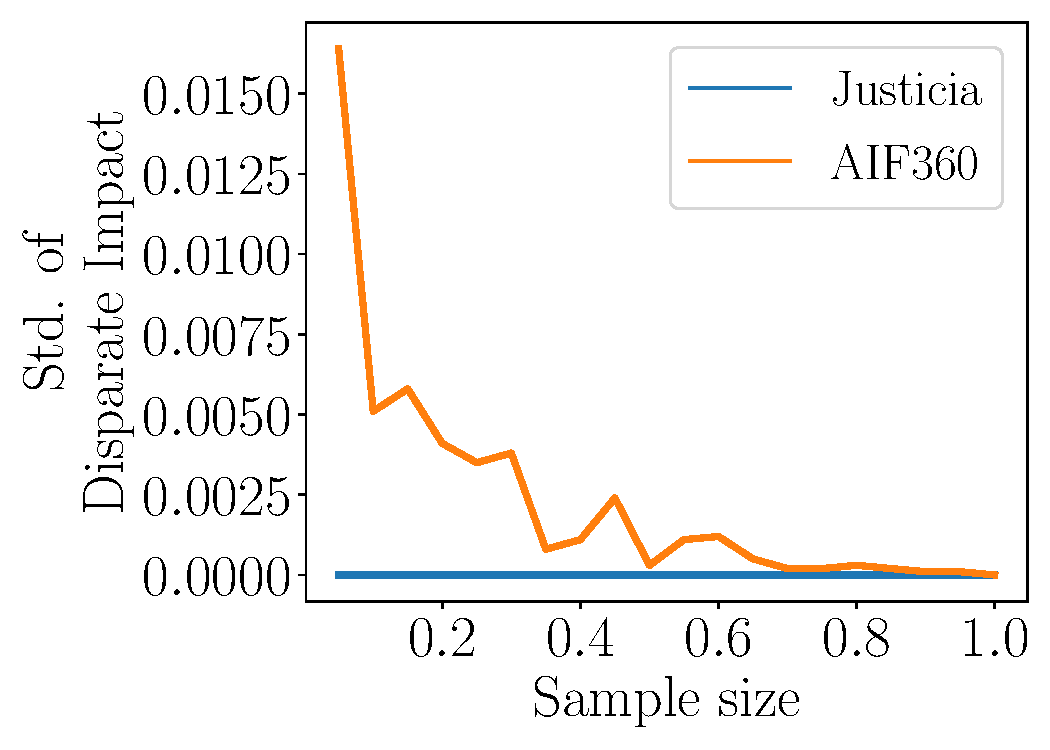
\includegraphics[scale=.5]{figures/sampling_DI_after_Compas_op_DT_race.pdf}
		} \hfil  
		\subfloat{
			\includegraphics[scale=.5]{figures/sampling_DI_before_Compas_op_LR_race.pdf}
		}
		\subfloat{
			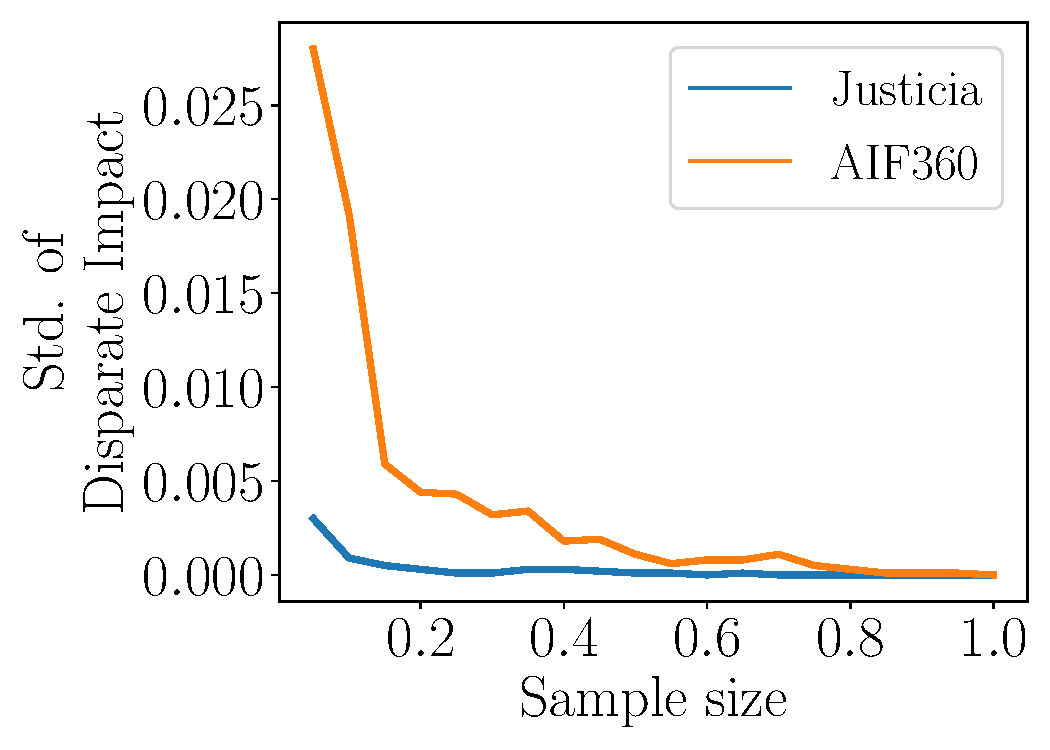
\includegraphics[scale=.5]{figures/sampling_DI_after_Compas_op_LR_race.pdf}
		} \hfil  
		
		
		
		
		\subfloat{
			\includegraphics[scale=.5]{figures/sampling_DI_before_Compas_op_DT_sex.pdf}
		}
		\subfloat{
			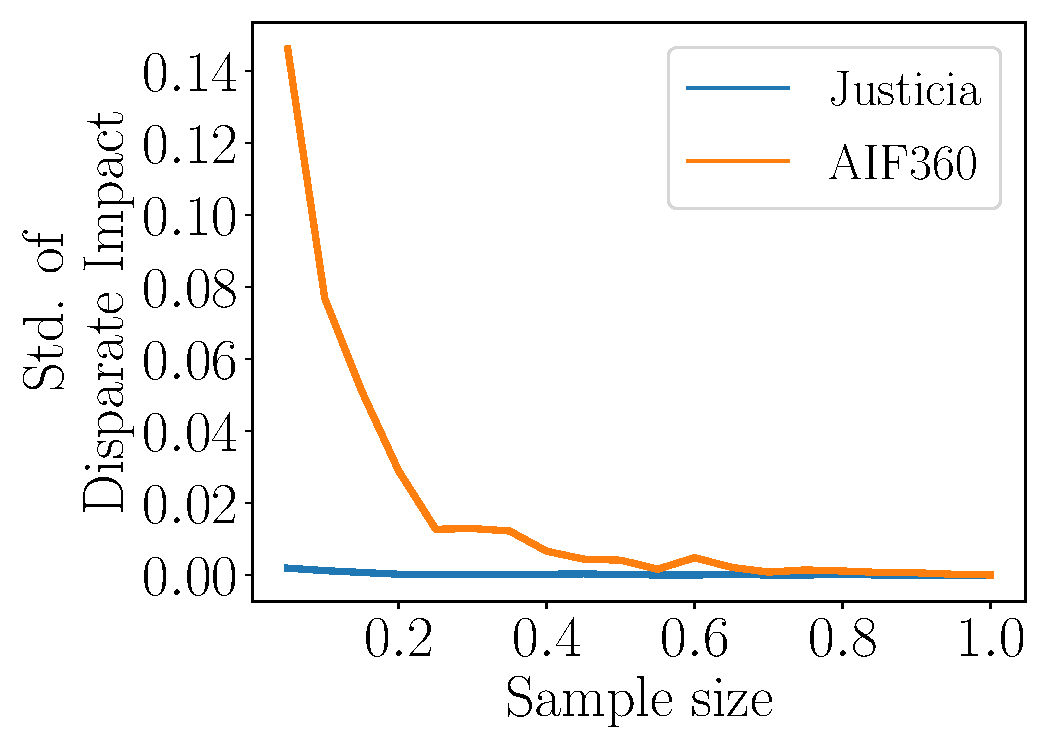
\includegraphics[scale=.5]{figures/sampling_DI_after_Compas_op_DT_sex.pdf}
		} \hfil
		
		\subfloat{
			\includegraphics[scale=.5]{figures/sampling_DI_before_Compas_op_LR_sex.pdf}
		}
		\subfloat{
			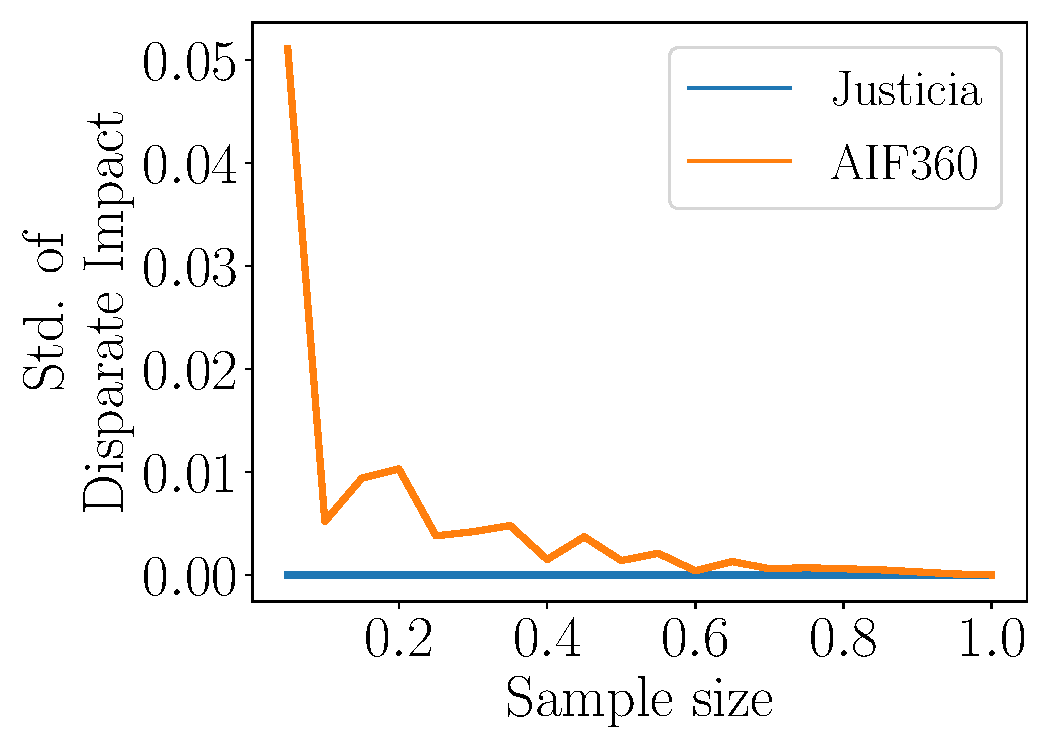
\includegraphics[scale=.5]{figures/sampling_DI_after_Compas_op_LR_sex.pdf}
		} \hfil
		
	\end{center}
	
	\caption{Effect of sampling.} 
\end{figure*}

\begin{figure*}
	\begin{center}
		\subfloat{
			\includegraphics[scale=.5]{figures/sampling_DI_before_German_op_DT_age.pdf}
		}
		\subfloat{
			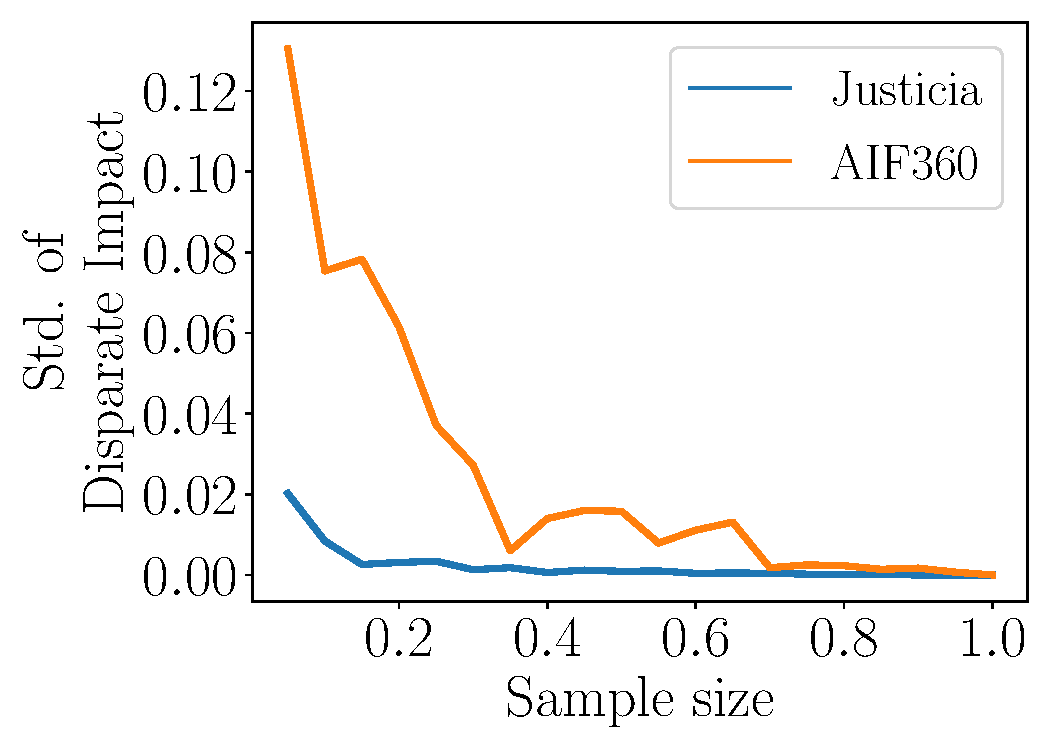
\includegraphics[scale=.5]{figures/sampling_DI_after_German_op_DT_age.pdf}
		} \hfil  
		\subfloat{
			\includegraphics[scale=.5]{figures/sampling_DI_before_German_op_LR_age.pdf}
		}
		\subfloat{
			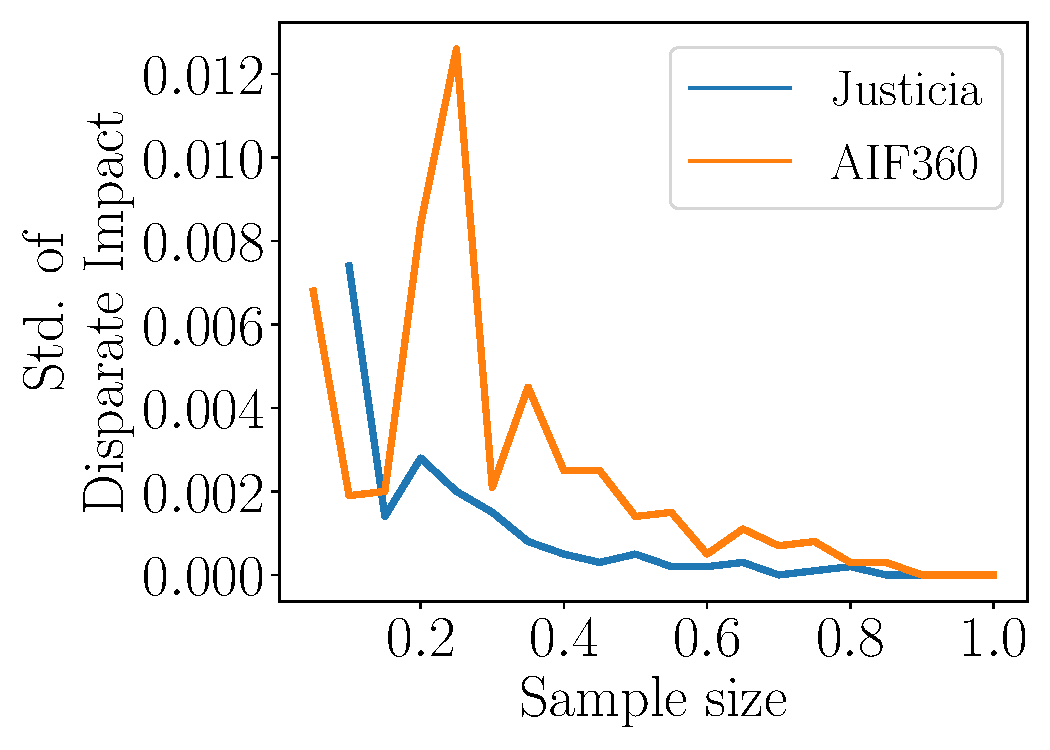
\includegraphics[scale=.5]{figures/sampling_DI_after_German_op_LR_age.pdf}
		} \hfil  
		
		
		
		
		\subfloat{
			\includegraphics[scale=.5]{figures/sampling_DI_before_German_op_DT_sex.pdf}
		}
		\subfloat{
			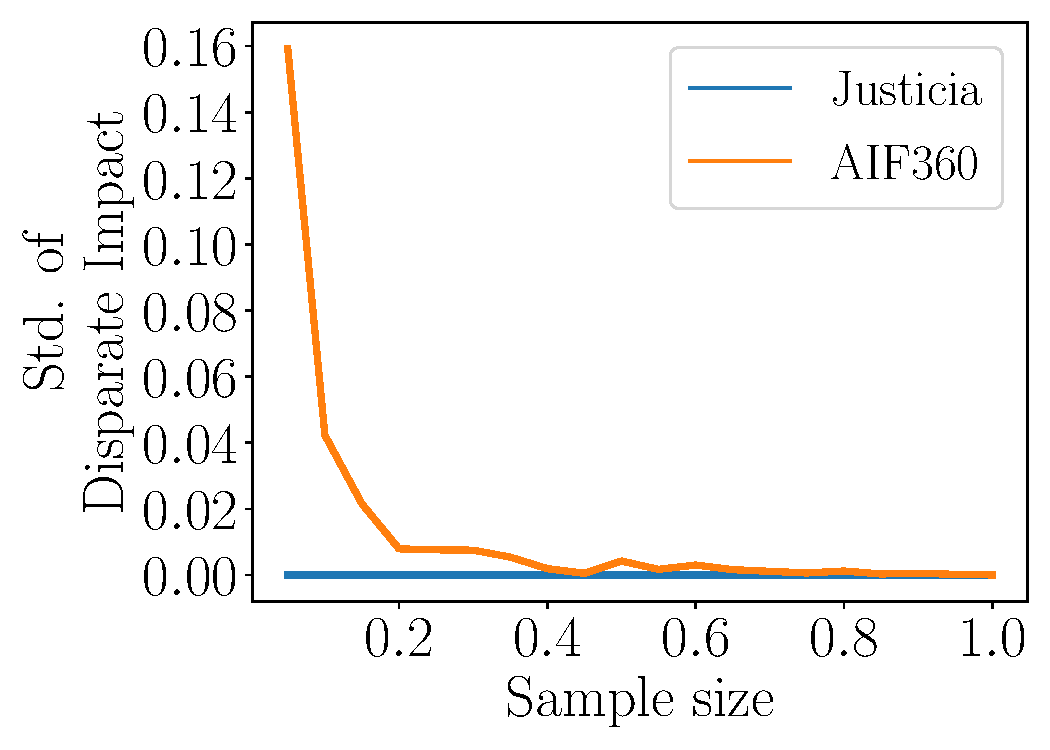
\includegraphics[scale=.5]{figures/sampling_DI_after_German_op_DT_sex.pdf}
		} \hfil
		
		\subfloat{
			\includegraphics[scale=.5]{figures/sampling_DI_before_German_op_LR_sex.pdf}
		}
		\subfloat{
			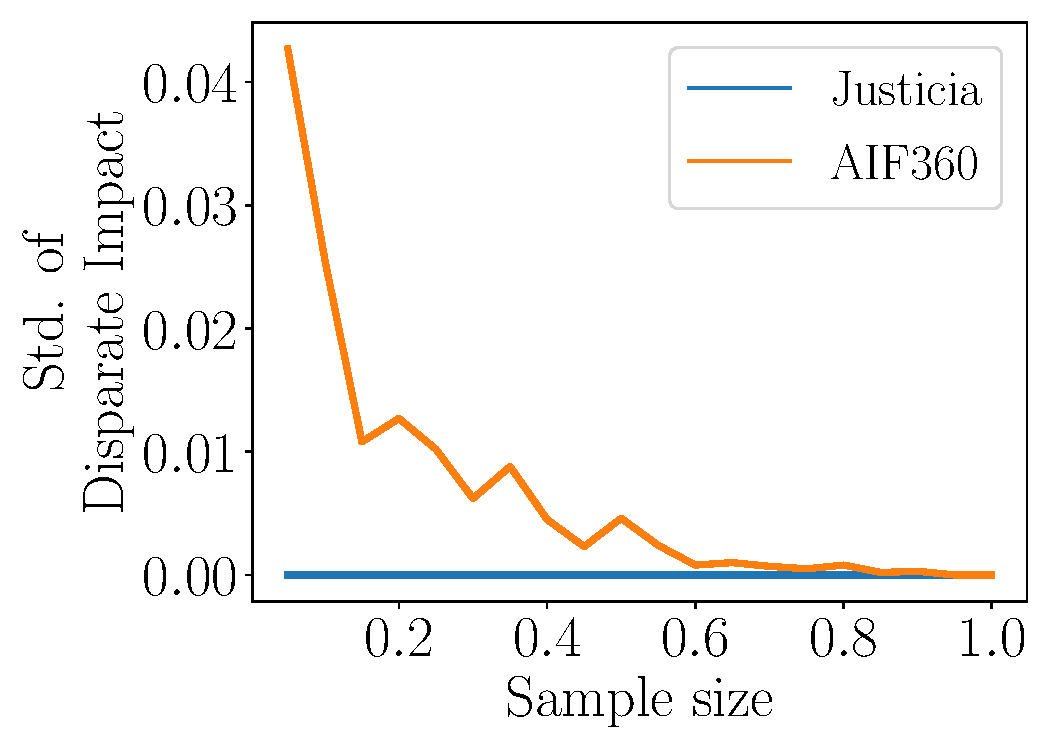
\includegraphics[scale=.5]{figures/sampling_DI_after_German_op_LR_sex.pdf}
		} \hfil
		
	\end{center}
	
	\caption{Effect of sampling.} 
\end{figure*}





\begin{figure*}
	\begin{center}
		\subfloat{
			\includegraphics[scale=.5]{figures/DI_Adult_rw_DT_race.pdf}
		}
		\subfloat{
			\includegraphics[scale=.5]{figures/SPD_Adult_rw_DT_race.pdf}
		} \hfil  
		\subfloat{
			\includegraphics[scale=.5]{figures/DI_Adult_rw_LR_race.pdf}
		}
		\subfloat{
			\includegraphics[scale=.5]{figures/SPD_Adult_rw_LR_race.pdf}
		} \hfil  
		
		
		
		
		\subfloat{
			\includegraphics[scale=.5]{figures/DI_Adult_rw_DT_sex.pdf}
		}
		\subfloat{
			\includegraphics[scale=.5]{figures/SPD_Adult_rw_DT_sex.pdf}
		} \hfil
		
		\subfloat{
			\includegraphics[scale=.5]{figures/DI_Adult_rw_LR_sex.pdf}
		}
		\subfloat{
			\includegraphics[scale=.5]{figures/SPD_Adult_rw_LR_sex.pdf}
		} \hfil
		
	\end{center}
	
	\caption{Result for applying reweighing (rw) algorithm on Adult dataset. We show results for three verifiers: RE-SSAT encoding with correlation (RE-cor), RE-SSAT encoding without correlation (RE), and statistical tool AIF360 and for two classifiers: decision tree (DT) and logistic regression (LR). If the preprocessing algorithm is successful, we observe an increase in disparate impact and a decrease in statistical parity difference as we apply the fairness algorithm. RE-cor and RE finds instances where the preprocessing algorithm fails to mitigate bias in the dataset.} 
\end{figure*}

\begin{figure*}
	\begin{center}
		
		
		\subfloat{
			\includegraphics[scale=.5]{figures/DI_German_rw_DT_age.pdf}
		}
		\subfloat{
			\includegraphics[scale=.5]{figures/SPD_German_rw_DT_age.pdf}
		} \hfil 
		
		\subfloat{
			\includegraphics[scale=.5]{figures/DI_German_rw_LR_age.pdf}
		}
		\subfloat{
			\includegraphics[scale=.5]{figures/SPD_German_rw_LR_age.pdf}
		} \hfil 
		
		
		\subfloat{
			\includegraphics[scale=.5]{figures/DI_German_rw_DT_sex.pdf}
		}
		\subfloat{
			\includegraphics[scale=.5]{figures/SPD_German_rw_DT_sex.pdf}
		} \hfil
		
		\subfloat{
			\includegraphics[scale=.5]{figures/DI_German_rw_LR_sex.pdf}
		}
		\subfloat{
			\includegraphics[scale=.5]{figures/SPD_German_rw_LR_sex.pdf}
		} \hfil
		
		
	\end{center}
	
	\caption{Result for applying reweighing (rw) algorithm on German-credit dataset. We show results for three verifiers: RE-SSAT encoding with correlation (RE-cor), RE-SSAT encoding without correlation (RE), and statistical tool AIF360 and for two classifiers: decision tree (DT) and logistic regression (LR). If the preprocessing algorithm is successful, we observe an increase in disparate impact and a decrease in statistical parity difference as we apply the fairness algorithm. RE-cor and RE finds instances where the preprocessing algorithm fails to mitigate bias in the dataset.} 
\end{figure*}

\begin{figure*}
	\begin{center}
		
		
		\subfloat{
			\includegraphics[scale=.5]{figures/DI_Compas_rw_DT_race.pdf}
		}
		\subfloat{
			\includegraphics[scale=.5]{figures/SPD_Compas_rw_DT_race.pdf}
		} \hfil 
		
		\subfloat{
			\includegraphics[scale=.5]{figures/DI_Compas_rw_LR_race.pdf}
		}
		\subfloat{
			\includegraphics[scale=.5]{figures/SPD_Compas_rw_LR_race.pdf}
		} \hfil
		
		\subfloat{
			\includegraphics[scale=.5]{figures/DI_Compas_rw_DT_sex.pdf}
		}
		\subfloat{
			\includegraphics[scale=.5]{figures/SPD_Compas_rw_DT_sex.pdf}
		} \hfil
		
		\subfloat{
			\includegraphics[scale=.5]{figures/DI_Compas_rw_LR_sex.pdf}
		}
		\subfloat{
			\includegraphics[scale=.5]{figures/SPD_Compas_rw_LR_sex.pdf}
		} \hfil
		
	\end{center}
	
	\caption{Result for applying reweighing (rw) algorithm on Compas dataset. We show results for three verifiers: RE-SSAT encoding with correlation (RE-cor), RE-SSAT encoding without correlation (RE), and statistical tool AIF360 and for two classifiers: decision tree (DT) and logistic regression (LR). If the preprocessing algorithm is successful, we observe an increase in disparate impact and a decrease in statistical parity difference as we apply the fairness algorithm. RE-cor and RE finds instances where the preprocessing algorithm fails to mitigate bias in the dataset.} 
\end{figure*}





\begin{figure*}
	\begin{center}
		\subfloat{
			\includegraphics[scale=.5]{figures/sampling_DI_before_Adult_rw_DT_race.pdf}
		}
		\subfloat{
			\includegraphics[scale=.5]{figures/sampling_DI_after_Adult_rw_DT_race.pdf}
		} \hfil  
		\subfloat{
			\includegraphics[scale=.5]{figures/sampling_DI_before_Adult_rw_LR_race.pdf}
		}
		\subfloat{
			\includegraphics[scale=.5]{figures/sampling_DI_after_Adult_rw_LR_race.pdf}
		} \hfil  
		
		
		
		
		\subfloat{
			\includegraphics[scale=.5]{figures/sampling_DI_before_Adult_rw_DT_sex.pdf}
		}
		\subfloat{
			\includegraphics[scale=.5]{figures/sampling_DI_after_Adult_rw_DT_sex.pdf}
		} \hfil
		
		\subfloat{
			\includegraphics[scale=.5]{figures/sampling_DI_before_Adult_rw_LR_sex.pdf}
		}
		\subfloat{
			\includegraphics[scale=.5]{figures/sampling_DI_after_Adult_rw_LR_sex.pdf}
		} \hfil
		
	\end{center}
	
	\caption{Effect of sampling.} 
\end{figure*}

\begin{figure*}
	\begin{center}
		\subfloat{
			\includegraphics[scale=.5]{figures/sampling_DI_before_Compas_rw_DT_race.pdf}
		}
		\subfloat{
			\includegraphics[scale=.5]{figures/sampling_DI_after_Compas_rw_DT_race.pdf}
		} \hfil  
		\subfloat{
			\includegraphics[scale=.5]{figures/sampling_DI_before_Compas_rw_LR_race.pdf}
		}
		\subfloat{
			\includegraphics[scale=.5]{figures/sampling_DI_after_Compas_rw_LR_race.pdf}
		} \hfil  
		
		
		
		
		\subfloat{
			\includegraphics[scale=.5]{figures/sampling_DI_before_Compas_rw_DT_sex.pdf}
		}
		\subfloat{
			\includegraphics[scale=.5]{figures/sampling_DI_after_Compas_rw_DT_sex.pdf}
		} \hfil
		
		\subfloat{
			\includegraphics[scale=.5]{figures/sampling_DI_before_Compas_rw_LR_sex.pdf}
		}
		\subfloat{
			\includegraphics[scale=.5]{figures/sampling_DI_after_Compas_rw_LR_sex.pdf}
		} \hfil
		
	\end{center}
	
	\caption{Effect of sampling.} 
\end{figure*}

\begin{figure*}
	\begin{center}
		\subfloat{
			\includegraphics[scale=.5]{figures/sampling_DI_before_German_rw_DT_age.pdf}
		}
		\subfloat{
			\includegraphics[scale=.5]{figures/sampling_DI_after_German_rw_DT_age.pdf}
		} \hfil  
		\subfloat{
			\includegraphics[scale=.5]{figures/sampling_DI_before_German_rw_LR_age.pdf}
		}
		\subfloat{
			\includegraphics[scale=.5]{figures/sampling_DI_after_German_rw_LR_age.pdf}
		} \hfil  
		
		
		
		
		\subfloat{
			\includegraphics[scale=.5]{figures/sampling_DI_before_German_rw_DT_sex.pdf}
		}
		\subfloat{
			\includegraphics[scale=.5]{figures/sampling_DI_after_German_rw_DT_sex.pdf}
		} \hfil
		
		\subfloat{
			\includegraphics[scale=.5]{figures/sampling_DI_before_German_rw_LR_sex.pdf}
		}
		\subfloat{
			\includegraphics[scale=.5]{figures/sampling_DI_after_German_rw_LR_sex.pdf}
		} \hfil
		
	\end{center}
	
	\caption{Effect of sampling.} 
\end{figure*}

\begin{figure*}
	\includegraphics[width=.23\linewidth]{figures/equivalence_di_adult_dt_age.pdf}
	\includegraphics[width=.23\linewidth]{figures/equivalence_di_adult_dt_race, age.pdf}
	\includegraphics[width=.23\linewidth]{figures/equivalence_di_adult_dt_race, sex, age.pdf}
	\includegraphics[width=.23\linewidth]{figures/equivalence_di_adult_dt_race, sex.pdf}
	\includegraphics[width=.23\linewidth]{figures/equivalence_di_adult_dt_race.pdf}
	\includegraphics[width=.23\linewidth]{figures/equivalence_di_adult_dt_sex, age.pdf}
	\includegraphics[width=.23\linewidth]{figures/equivalence_di_adult_dt_sex.pdf}
	\includegraphics[width=.23\linewidth]{figures/equivalence_di_adult_lr_age.pdf}
	\includegraphics[width=.23\linewidth]{figures/equivalence_di_adult_lr_race, age.pdf}
	\includegraphics[width=.23\linewidth]{figures/equivalence_di_adult_lr_race, sex, age.pdf}
	\includegraphics[width=.23\linewidth]{figures/equivalence_di_adult_lr_race, sex.pdf}
	\includegraphics[width=.23\linewidth]{figures/equivalence_di_adult_lr_race.pdf}
	\includegraphics[width=.23\linewidth]{figures/equivalence_di_adult_lr_sex, age.pdf}
	\includegraphics[width=.23\linewidth]{figures/equivalence_di_adult_lr_sex.pdf}
	\includegraphics[width=.23\linewidth]{figures/equivalence_di_adult_mlic_age.pdf}
	\includegraphics[width=.23\linewidth]{figures/equivalence_di_adult_mlic_race, age.pdf}
	\includegraphics[width=.23\linewidth]{figures/equivalence_di_adult_mlic_race, sex, age.pdf}
	\includegraphics[width=.23\linewidth]{figures/equivalence_di_adult_mlic_race, sex.pdf}
	\includegraphics[width=.23\linewidth]{figures/equivalence_di_adult_mlic_race.pdf}
	\includegraphics[width=.23\linewidth]{figures/equivalence_di_adult_mlic_sex, age.pdf}
	\includegraphics[width=.23\linewidth]{figures/equivalence_di_adult_mlic_sex.pdf}
\end{figure*}


\begin{figure*}
\includegraphics[width=0.23\linewidth]{figures/equivalence_spd_adult_dt_age.pdf}
\includegraphics[width=0.23\linewidth]{figures/equivalence_spd_adult_dt_race, age.pdf}
\includegraphics[width=0.23\linewidth]{figures/equivalence_spd_adult_dt_race, sex, age.pdf}
\includegraphics[width=0.23\linewidth]{figures/equivalence_spd_adult_dt_race, sex.pdf}
\includegraphics[width=0.23\linewidth]{figures/equivalence_spd_adult_dt_race.pdf}
\includegraphics[width=0.23\linewidth]{figures/equivalence_spd_adult_dt_sex, age.pdf}
\includegraphics[width=0.23\linewidth]{figures/equivalence_spd_adult_dt_sex.pdf}
\includegraphics[width=0.23\linewidth]{figures/equivalence_spd_adult_lr_age.pdf}
\includegraphics[width=0.23\linewidth]{figures/equivalence_spd_adult_lr_race, age.pdf}
\includegraphics[width=0.23\linewidth]{figures/equivalence_spd_adult_lr_race, sex, age.pdf}
\includegraphics[width=0.23\linewidth]{figures/equivalence_spd_adult_lr_race, sex.pdf}
\includegraphics[width=0.23\linewidth]{figures/equivalence_spd_adult_lr_race.pdf}
\includegraphics[width=0.23\linewidth]{figures/equivalence_spd_adult_lr_sex, age.pdf}
\includegraphics[width=0.23\linewidth]{figures/equivalence_spd_adult_lr_sex.pdf}
\includegraphics[width=0.23\linewidth]{figures/equivalence_spd_adult_mlic_age.pdf}
\includegraphics[width=0.23\linewidth]{figures/equivalence_spd_adult_mlic_race, age.pdf}
\includegraphics[width=0.23\linewidth]{figures/equivalence_spd_adult_mlic_race, sex, age.pdf}
\includegraphics[width=0.23\linewidth]{figures/equivalence_spd_adult_mlic_race, sex.pdf}
\includegraphics[width=0.23\linewidth]{figures/equivalence_spd_adult_mlic_race.pdf}
\includegraphics[width=0.23\linewidth]{figures/equivalence_spd_adult_mlic_sex, age.pdf}
\includegraphics[width=0.23\linewidth]{figures/equivalence_spd_adult_mlic_sex.pdf}
\end{figure*}


\begin{figure*}
	\includegraphics[width=0.23\linewidth]{figures/equivalence_di_german_dt_age, sex.pdf}
	\includegraphics[width=0.23\linewidth]{figures/equivalence_di_german_dt_age.pdf}
	\includegraphics[width=0.23\linewidth]{figures/equivalence_di_german_dt_sex.pdf}
	\includegraphics[width=0.23\linewidth]{figures/equivalence_di_german_lr_age, sex.pdf}
	\includegraphics[width=0.23\linewidth]{figures/equivalence_di_german_lr_age.pdf}
	\includegraphics[width=0.23\linewidth]{figures/equivalence_di_german_lr_sex.pdf}
	\includegraphics[width=0.23\linewidth]{figures/equivalence_di_german_mlic_age, sex.pdf}
	\includegraphics[width=0.23\linewidth]{figures/equivalence_di_german_mlic_age.pdf}
	\includegraphics[width=0.23\linewidth]{figures/equivalence_di_german_mlic_sex.pdf}
	

\end{figure*}

\begin{figure*}
		\includegraphics[width=0.23\linewidth]{figures/equivalence_spd_german_dt_age, sex.pdf}
	\includegraphics[width=0.23\linewidth]{figures/equivalence_spd_german_dt_age.pdf}
	\includegraphics[width=0.23\linewidth]{figures/equivalence_spd_german_dt_sex.pdf}
	\includegraphics[width=0.23\linewidth]{figures/equivalence_spd_german_lr_age, sex.pdf}
	\includegraphics[width=0.23\linewidth]{figures/equivalence_spd_german_lr_age.pdf}
	\includegraphics[width=0.23\linewidth]{figures/equivalence_spd_german_lr_sex.pdf}
	\includegraphics[width=0.23\linewidth]{figures/equivalence_spd_german_mlic_age, sex.pdf}
	\includegraphics[width=0.23\linewidth]{figures/equivalence_spd_german_mlic_age.pdf}
	\includegraphics[width=0.23\linewidth]{figures/equivalence_spd_german_mlic_sex.pdf}
	
\end{figure*}

\begin{figure*}
	\includegraphics[width=0.23\linewidth]{figures/equivalence_di_titanic_dt_age.pdf}
	\includegraphics[width=0.23\linewidth]{figures/equivalence_di_titanic_dt_passenger class, age.pdf}
	\includegraphics[width=0.23\linewidth]{figures/equivalence_di_titanic_dt_passenger class.pdf}
	\includegraphics[width=0.23\linewidth]{figures/equivalence_di_titanic_dt_sex, age.pdf}
	\includegraphics[width=0.23\linewidth]{figures/equivalence_di_titanic_dt_sex, passenger class, age.pdf}
	\includegraphics[width=0.23\linewidth]{figures/equivalence_di_titanic_dt_sex, passenger class.pdf}
	\includegraphics[width=0.23\linewidth]{figures/equivalence_di_titanic_dt_sex.pdf}
	\includegraphics[width=0.23\linewidth]{figures/equivalence_di_titanic_lr_age.pdf}
	\includegraphics[width=0.23\linewidth]{figures/equivalence_di_titanic_lr_passenger class, age.pdf}
	\includegraphics[width=0.23\linewidth]{figures/equivalence_di_titanic_lr_passenger class.pdf}
	\includegraphics[width=0.23\linewidth]{figures/equivalence_di_titanic_lr_sex, age.pdf}
	\includegraphics[width=0.23\linewidth]{figures/equivalence_di_titanic_lr_sex, passenger class, age.pdf}
	\includegraphics[width=0.23\linewidth]{figures/equivalence_di_titanic_lr_sex, passenger class.pdf}
	\includegraphics[width=0.23\linewidth]{figures/equivalence_di_titanic_lr_sex.pdf}
	\includegraphics[width=0.23\linewidth]{figures/equivalence_di_titanic_mlic_age.pdf}
	\includegraphics[width=0.23\linewidth]{figures/equivalence_di_titanic_mlic_passenger class, age.pdf}
	\includegraphics[width=0.23\linewidth]{figures/equivalence_di_titanic_mlic_passenger class.pdf}
	\includegraphics[width=0.23\linewidth]{figures/equivalence_di_titanic_mlic_sex, age.pdf}
	\includegraphics[width=0.23\linewidth]{figures/equivalence_di_titanic_mlic_sex, passenger class, age.pdf}
	\includegraphics[width=0.23\linewidth]{figures/equivalence_di_titanic_mlic_sex, passenger class.pdf}
	\includegraphics[width=0.23\linewidth]{figures/equivalence_di_titanic_mlic_sex.pdf}
	
\end{figure*}

\begin{figure*}
	\includegraphics[width=0.23\linewidth]{figures/equivalence_spd_titanic_dt_age.pdf}
	\includegraphics[width=0.23\linewidth]{figures/equivalence_spd_titanic_dt_passenger class, age.pdf}
	\includegraphics[width=0.23\linewidth]{figures/equivalence_spd_titanic_dt_passenger class.pdf}
	\includegraphics[width=0.23\linewidth]{figures/equivalence_spd_titanic_dt_sex, age.pdf}
	\includegraphics[width=0.23\linewidth]{figures/equivalence_spd_titanic_dt_sex, passenger class, age.pdf}
	\includegraphics[width=0.23\linewidth]{figures/equivalence_spd_titanic_dt_sex, passenger class.pdf}
	\includegraphics[width=0.23\linewidth]{figures/equivalence_spd_titanic_dt_sex.pdf}
	\includegraphics[width=0.23\linewidth]{figures/equivalence_spd_titanic_lr_age.pdf}
	\includegraphics[width=0.23\linewidth]{figures/equivalence_spd_titanic_lr_passenger class, age.pdf}
	\includegraphics[width=0.23\linewidth]{figures/equivalence_spd_titanic_lr_passenger class.pdf}
	\includegraphics[width=0.23\linewidth]{figures/equivalence_spd_titanic_lr_sex, age.pdf}
	\includegraphics[width=0.23\linewidth]{figures/equivalence_spd_titanic_lr_sex, passenger class, age.pdf}
	\includegraphics[width=0.23\linewidth]{figures/equivalence_spd_titanic_lr_sex, passenger class.pdf}
	\includegraphics[width=0.23\linewidth]{figures/equivalence_spd_titanic_lr_sex.pdf}
	\includegraphics[width=0.23\linewidth]{figures/equivalence_spd_titanic_mlic_age.pdf}
	\includegraphics[width=0.23\linewidth]{figures/equivalence_spd_titanic_mlic_passenger class, age.pdf}
	\includegraphics[width=0.23\linewidth]{figures/equivalence_spd_titanic_mlic_passenger class.pdf}
	\includegraphics[width=0.23\linewidth]{figures/equivalence_spd_titanic_mlic_sex, age.pdf}
	\includegraphics[width=0.23\linewidth]{figures/equivalence_spd_titanic_mlic_sex, passenger class, age.pdf}
	\includegraphics[width=0.23\linewidth]{figures/equivalence_spd_titanic_mlic_sex, passenger class.pdf}
	\includegraphics[width=0.23\linewidth]{figures/equivalence_spd_titanic_mlic_sex.pdf}
\end{figure*}



\begin{figure*}
	\includegraphics[width=0.23\linewidth]{figures/encoding_runtime_adult_dt.pdf}
	\includegraphics[width=0.23\linewidth]{figures/encoding_runtime_adult_lr.pdf}
	\includegraphics[width=0.23\linewidth]{figures/encoding_runtime_adult_mlic.pdf}
	\includegraphics[width=0.23\linewidth]{figures/encoding_runtime_german_dt.pdf}
	\includegraphics[width=0.23\linewidth]{figures/encoding_runtime_german_lr.pdf}
	\includegraphics[width=0.23\linewidth]{figures/encoding_runtime_german_mlic.pdf}
	\includegraphics[width=0.23\linewidth]{figures/encoding_runtime_ricci_dt.pdf}
	\includegraphics[width=0.23\linewidth]{figures/encoding_runtime_ricci_lr.pdf}
	\includegraphics[width=0.23\linewidth]{figures/encoding_runtime_ricci_mlic.pdf}
	\includegraphics[width=0.23\linewidth]{figures/encoding_runtime_titanic_dt.pdf}
	\includegraphics[width=0.23\linewidth]{figures/encoding_runtime_titanic_lr.pdf}
	\includegraphics[width=0.23\linewidth]{figures/encoding_runtime_titanic_mlic.pdf}
\end{figure*}


\begin{figure*}
\includegraphics[width=0.23\linewidth]{figures/sensitive_attribute_age_di_adult_dt_RE.pdf}
\includegraphics[width=0.23\linewidth]{figures/sensitive_attribute_age_di_adult_lr_RE.pdf}
\includegraphics[width=0.23\linewidth]{figures/sensitive_attribute_age_di_adult_mlic_RE.pdf}
\includegraphics[width=0.23\linewidth]{figures/sensitive_attribute_age_spd_adult_dt_RE.pdf}
\includegraphics[width=0.23\linewidth]{figures/sensitive_attribute_age_spd_adult_lr_RE.pdf}
\includegraphics[width=0.23\linewidth]{figures/sensitive_attribute_age_spd_adult_mlic_RE.pdf}
\includegraphics[width=0.23\linewidth]{figures/sensitive_attribute_race_di_adult_dt_RE.pdf}
\includegraphics[width=0.23\linewidth]{figures/sensitive_attribute_race_di_adult_lr_RE.pdf}
\includegraphics[width=0.23\linewidth]{figures/sensitive_attribute_race_di_adult_mlic_RE.pdf}
\includegraphics[width=0.23\linewidth]{figures/sensitive_attribute_race_spd_adult_dt_RE.pdf}
\includegraphics[width=0.23\linewidth]{figures/sensitive_attribute_race_spd_adult_lr_RE.pdf}
\includegraphics[width=0.23\linewidth]{figures/sensitive_attribute_race_spd_adult_mlic_RE.pdf}
\includegraphics[width=0.23\linewidth]{figures/sensitive_attribute_sex_di_adult_dt_RE.pdf}
\includegraphics[width=0.23\linewidth]{figures/sensitive_attribute_sex_di_adult_lr_RE.pdf}
\includegraphics[width=0.23\linewidth]{figures/sensitive_attribute_sex_di_adult_mlic_RE.pdf}
\includegraphics[width=0.23\linewidth]{figures/sensitive_attribute_sex_spd_adult_dt_RE.pdf}
\includegraphics[width=0.23\linewidth]{figures/sensitive_attribute_sex_spd_adult_lr_RE.pdf}
\includegraphics[width=0.23\linewidth]{figures/sensitive_attribute_sex_spd_adult_mlic_RE.pdf}
\end{figure*}


\begin{figure*}
	\includegraphics[width=0.23\linewidth]{figures/sensitive_attribute_age_di_adult_dt_RE(cor).pdf}
	\includegraphics[width=0.23\linewidth]{figures/sensitive_attribute_age_di_adult_lr_RE(cor).pdf}
	\includegraphics[width=0.23\linewidth]{figures/sensitive_attribute_age_di_adult_mlic_RE(cor).pdf}
	\includegraphics[width=0.23\linewidth]{figures/sensitive_attribute_age_spd_adult_dt_RE(cor).pdf}
	\includegraphics[width=0.23\linewidth]{figures/sensitive_attribute_age_spd_adult_lr_RE(cor).pdf}
	\includegraphics[width=0.23\linewidth]{figures/sensitive_attribute_age_spd_adult_mlic_RE(cor).pdf}
	\includegraphics[width=0.23\linewidth]{figures/sensitive_attribute_race_di_adult_dt_RE(cor).pdf}
	\includegraphics[width=0.23\linewidth]{figures/sensitive_attribute_race_di_adult_lr_RE(cor).pdf}
	\includegraphics[width=0.23\linewidth]{figures/sensitive_attribute_race_di_adult_mlic_RE(cor).pdf}
	\includegraphics[width=0.23\linewidth]{figures/sensitive_attribute_race_spd_adult_dt_RE(cor).pdf}
	\includegraphics[width=0.23\linewidth]{figures/sensitive_attribute_race_spd_adult_lr_RE(cor).pdf}
	\includegraphics[width=0.23\linewidth]{figures/sensitive_attribute_race_spd_adult_mlic_RE(cor).pdf}
	\includegraphics[width=0.23\linewidth]{figures/sensitive_attribute_sex_di_adult_dt_RE(cor).pdf}
	\includegraphics[width=0.23\linewidth]{figures/sensitive_attribute_sex_di_adult_lr_RE(cor).pdf}
	\includegraphics[width=0.23\linewidth]{figures/sensitive_attribute_sex_di_adult_mlic_RE(cor).pdf}
	\includegraphics[width=0.23\linewidth]{figures/sensitive_attribute_sex_spd_adult_dt_RE(cor).pdf}
	\includegraphics[width=0.23\linewidth]{figures/sensitive_attribute_sex_spd_adult_lr_RE(cor).pdf}
	\includegraphics[width=0.23\linewidth]{figures/sensitive_attribute_sex_spd_adult_mlic_RE(cor).pdf}
\end{figure*}


\begin{figure*}
	\includegraphics[width=0.23\linewidth]{figures/sensitive_attribute_age_di_german_dt_RE(cor).pdf}
	\includegraphics[width=0.23\linewidth]{figures/sensitive_attribute_age_di_german_dt_RE.pdf}
	\includegraphics[width=0.23\linewidth]{figures/sensitive_attribute_age_di_german_lr_RE(cor).pdf}
	\includegraphics[width=0.23\linewidth]{figures/sensitive_attribute_age_di_german_lr_RE.pdf}
	\includegraphics[width=0.23\linewidth]{figures/sensitive_attribute_age_di_german_mlic_RE(cor).pdf}
	\includegraphics[width=0.23\linewidth]{figures/sensitive_attribute_age_di_german_mlic_RE.pdf}
	\includegraphics[width=0.23\linewidth]{figures/sensitive_attribute_age_spd_german_dt_RE(cor).pdf}
	\includegraphics[width=0.23\linewidth]{figures/sensitive_attribute_age_spd_german_dt_RE.pdf}
	\includegraphics[width=0.23\linewidth]{figures/sensitive_attribute_age_spd_german_lr_RE(cor).pdf}
	\includegraphics[width=0.23\linewidth]{figures/sensitive_attribute_age_spd_german_lr_RE.pdf}
	\includegraphics[width=0.23\linewidth]{figures/sensitive_attribute_age_spd_german_mlic_RE(cor).pdf}
	\includegraphics[width=0.23\linewidth]{figures/sensitive_attribute_age_spd_german_mlic_RE.pdf}
	\includegraphics[width=0.23\linewidth]{figures/sensitive_attribute_sex_di_german_dt_RE(cor).pdf}
	\includegraphics[width=0.23\linewidth]{figures/sensitive_attribute_sex_di_german_dt_RE.pdf}
	\includegraphics[width=0.23\linewidth]{figures/sensitive_attribute_sex_di_german_lr_RE(cor).pdf}
	\includegraphics[width=0.23\linewidth]{figures/sensitive_attribute_sex_di_german_lr_RE.pdf}
	\includegraphics[width=0.23\linewidth]{figures/sensitive_attribute_sex_di_german_mlic_RE(cor).pdf}
	\includegraphics[width=0.23\linewidth]{figures/sensitive_attribute_sex_di_german_mlic_RE.pdf}
	\includegraphics[width=0.23\linewidth]{figures/sensitive_attribute_sex_spd_german_dt_RE(cor).pdf}
	\includegraphics[width=0.23\linewidth]{figures/sensitive_attribute_sex_spd_german_dt_RE.pdf}
	\includegraphics[width=0.23\linewidth]{figures/sensitive_attribute_sex_spd_german_lr_RE(cor).pdf}
	\includegraphics[width=0.23\linewidth]{figures/sensitive_attribute_sex_spd_german_lr_RE.pdf}
	\includegraphics[width=0.23\linewidth]{figures/sensitive_attribute_sex_spd_german_mlic_RE(cor).pdf}
	\includegraphics[width=0.23\linewidth]{figures/sensitive_attribute_sex_spd_german_mlic_RE.pdf}
\end{figure*}


\begin{figure*}
	\includegraphics[width=0.23\linewidth]{figures/sensitive_attribute_age_di_titanic_dt_RE.pdf}
	\includegraphics[width=0.23\linewidth]{figures/sensitive_attribute_age_di_titanic_lr_RE.pdf}
	\includegraphics[width=0.23\linewidth]{figures/sensitive_attribute_age_di_titanic_mlic_RE.pdf}
	\includegraphics[width=0.23\linewidth]{figures/sensitive_attribute_age_spd_titanic_dt_RE.pdf}
	\includegraphics[width=0.23\linewidth]{figures/sensitive_attribute_age_spd_titanic_lr_RE.pdf}
	\includegraphics[width=0.23\linewidth]{figures/sensitive_attribute_age_spd_titanic_mlic_RE.pdf}
	\includegraphics[width=0.23\linewidth]{figures/sensitive_attribute_passenger class_di_titanic_dt_RE.pdf}
	\includegraphics[width=0.23\linewidth]{figures/sensitive_attribute_passenger class_di_titanic_lr_RE.pdf}
	\includegraphics[width=0.23\linewidth]{figures/sensitive_attribute_passenger class_di_titanic_mlic_RE.pdf}
	\includegraphics[width=0.23\linewidth]{figures/sensitive_attribute_passenger class_spd_titanic_dt_RE.pdf}
	\includegraphics[width=0.23\linewidth]{figures/sensitive_attribute_passenger class_spd_titanic_lr_RE.pdf}
	\includegraphics[width=0.23\linewidth]{figures/sensitive_attribute_passenger class_spd_titanic_mlic_RE.pdf}
	\includegraphics[width=0.23\linewidth]{figures/sensitive_attribute_sex_di_titanic_dt_RE.pdf}
	\includegraphics[width=0.23\linewidth]{figures/sensitive_attribute_sex_di_titanic_lr_RE.pdf}
	\includegraphics[width=0.23\linewidth]{figures/sensitive_attribute_sex_di_titanic_mlic_RE.pdf}
	\includegraphics[width=0.23\linewidth]{figures/sensitive_attribute_sex_spd_titanic_dt_RE.pdf}
	\includegraphics[width=0.23\linewidth]{figures/sensitive_attribute_sex_spd_titanic_lr_RE.pdf}
	\includegraphics[width=0.23\linewidth]{figures/sensitive_attribute_sex_spd_titanic_mlic_RE.pdf}
\end{figure*}


\begin{figure*}
	\includegraphics[width=0.23\linewidth]{figures/sensitive_attribute_age_di_titanic_dt_RE(cor).pdf}
	\includegraphics[width=0.23\linewidth]{figures/sensitive_attribute_age_di_titanic_lr_RE(cor).pdf}
	\includegraphics[width=0.23\linewidth]{figures/sensitive_attribute_age_di_titanic_mlic_RE(cor).pdf}
	\includegraphics[width=0.23\linewidth]{figures/sensitive_attribute_age_spd_titanic_dt_RE(cor).pdf}
	\includegraphics[width=0.23\linewidth]{figures/sensitive_attribute_age_spd_titanic_lr_RE(cor).pdf}
	\includegraphics[width=0.23\linewidth]{figures/sensitive_attribute_age_spd_titanic_mlic_RE(cor).pdf}
	\includegraphics[width=0.23\linewidth]{figures/sensitive_attribute_passenger class_di_titanic_dt_RE(cor).pdf}
	\includegraphics[width=0.23\linewidth]{figures/sensitive_attribute_passenger class_di_titanic_lr_RE(cor).pdf}
	\includegraphics[width=0.23\linewidth]{figures/sensitive_attribute_passenger class_di_titanic_mlic_RE(cor).pdf}
	\includegraphics[width=0.23\linewidth]{figures/sensitive_attribute_passenger class_spd_titanic_dt_RE(cor).pdf}
	\includegraphics[width=0.23\linewidth]{figures/sensitive_attribute_passenger class_spd_titanic_lr_RE(cor).pdf}
	\includegraphics[width=0.23\linewidth]{figures/sensitive_attribute_passenger class_spd_titanic_mlic_RE(cor).pdf}
	\includegraphics[width=0.23\linewidth]{figures/sensitive_attribute_sex_di_titanic_dt_RE(cor).pdf}
	\includegraphics[width=0.23\linewidth]{figures/sensitive_attribute_sex_di_titanic_lr_RE(cor).pdf}
	\includegraphics[width=0.23\linewidth]{figures/sensitive_attribute_sex_di_titanic_mlic_RE(cor).pdf}
	\includegraphics[width=0.23\linewidth]{figures/sensitive_attribute_sex_spd_titanic_dt_RE(cor).pdf}
	\includegraphics[width=0.23\linewidth]{figures/sensitive_attribute_sex_spd_titanic_lr_RE(cor).pdf}
	\includegraphics[width=0.23\linewidth]{figures/sensitive_attribute_sex_spd_titanic_mlic_RE(cor).pdf}
\end{figure*}


\begin{figure*}
	\includegraphics[width=0.23\linewidth]{figures/sensitive_attribute_Position_di_ricci_dt_RE(cor).pdf}
	\includegraphics[width=0.23\linewidth]{figures/sensitive_attribute_Position_di_ricci_dt_RE.pdf}
	\includegraphics[width=0.23\linewidth]{figures/sensitive_attribute_Position_di_ricci_lr_RE(cor).pdf}
	\includegraphics[width=0.23\linewidth]{figures/sensitive_attribute_Position_di_ricci_lr_RE.pdf}
	\includegraphics[width=0.23\linewidth]{figures/sensitive_attribute_Position_di_ricci_mlic_RE(cor).pdf}
	\includegraphics[width=0.23\linewidth]{figures/sensitive_attribute_Position_di_ricci_mlic_RE.pdf}
	\includegraphics[width=0.23\linewidth]{figures/sensitive_attribute_Position_spd_ricci_dt_RE(cor).pdf}
	\includegraphics[width=0.23\linewidth]{figures/sensitive_attribute_Position_spd_ricci_dt_RE.pdf}
	\includegraphics[width=0.23\linewidth]{figures/sensitive_attribute_Position_spd_ricci_lr_RE(cor).pdf}
	\includegraphics[width=0.23\linewidth]{figures/sensitive_attribute_Position_spd_ricci_lr_RE.pdf}
	\includegraphics[width=0.23\linewidth]{figures/sensitive_attribute_Position_spd_ricci_mlic_RE(cor).pdf}
	\includegraphics[width=0.23\linewidth]{figures/sensitive_attribute_Position_spd_ricci_mlic_RE.pdf}
	\includegraphics[width=0.23\linewidth]{figures/sensitive_attribute_Race_di_ricci_dt_RE(cor).pdf}
	\includegraphics[width=0.23\linewidth]{figures/sensitive_attribute_Race_di_ricci_dt_RE.pdf}
	\includegraphics[width=0.23\linewidth]{figures/sensitive_attribute_Race_di_ricci_lr_RE(cor).pdf}
	\includegraphics[width=0.23\linewidth]{figures/sensitive_attribute_Race_di_ricci_lr_RE.pdf}
	\includegraphics[width=0.23\linewidth]{figures/sensitive_attribute_Race_di_ricci_mlic_RE(cor).pdf}
	\includegraphics[width=0.23\linewidth]{figures/sensitive_attribute_Race_di_ricci_mlic_RE.pdf}
	\includegraphics[width=0.23\linewidth]{figures/sensitive_attribute_Race_spd_ricci_dt_RE(cor).pdf}
	\includegraphics[width=0.23\linewidth]{figures/sensitive_attribute_Race_spd_ricci_dt_RE.pdf}
	\includegraphics[width=0.23\linewidth]{figures/sensitive_attribute_Race_spd_ricci_lr_RE(cor).pdf}
	\includegraphics[width=0.23\linewidth]{figures/sensitive_attribute_Race_spd_ricci_lr_RE.pdf}
	\includegraphics[width=0.23\linewidth]{figures/sensitive_attribute_Race_spd_ricci_mlic_RE(cor).pdf}
	\includegraphics[width=0.23\linewidth]{figures/sensitive_attribute_Race_spd_ricci_mlic_RE.pdf}
\end{figure*}

\begin{figure*}
	\includegraphics[width=.235\linewidth]{figures/threshold_adult_lr_RE(cor)_age.pdf}
	\includegraphics[width=.235\linewidth]{figures/threshold_adult_lr_RE(cor)_race, age.pdf}
	\includegraphics[width=.235\linewidth]{figures/threshold_adult_lr_RE(cor)_race, sex, age.pdf}
	\includegraphics[width=.235\linewidth]{figures/threshold_adult_lr_RE(cor)_race, sex.pdf}
	\includegraphics[width=.235\linewidth]{figures/threshold_adult_lr_RE(cor)_race.pdf}
	\includegraphics[width=.235\linewidth]{figures/threshold_adult_lr_RE(cor)_sex, age.pdf}
	\includegraphics[width=.235\linewidth]{figures/threshold_adult_lr_RE(cor)_sex.pdf}
	\includegraphics[width=.235\linewidth]{figures/threshold_adult_lr_RE_age.pdf}
	\includegraphics[width=.235\linewidth]{figures/threshold_adult_lr_RE_race, age.pdf}
	\includegraphics[width=.235\linewidth]{figures/threshold_adult_lr_RE_race, sex, age.pdf}
	\includegraphics[width=.235\linewidth]{figures/threshold_adult_lr_RE_race, sex.pdf}
	\includegraphics[width=.235\linewidth]{figures/threshold_adult_lr_RE_race.pdf}
	\includegraphics[width=.235\linewidth]{figures/threshold_adult_lr_RE_sex, age.pdf}
	\includegraphics[width=.235\linewidth]{figures/threshold_adult_lr_RE_sex.pdf}

\end{figure*}

\begin{figure*}
	\includegraphics[width=.235\linewidth]{figures/threshold_german_lr_RE(cor)_age, sex.pdf}
	\includegraphics[width=.235\linewidth]{figures/threshold_german_lr_RE(cor)_age.pdf}
	\includegraphics[width=.235\linewidth]{figures/threshold_german_lr_RE(cor)_sex.pdf}
	\includegraphics[width=.235\linewidth]{figures/threshold_german_lr_RE_age, sex.pdf}
	\includegraphics[width=.235\linewidth]{figures/threshold_german_lr_RE_age.pdf}
	\includegraphics[width=.235\linewidth]{figures/threshold_german_lr_RE_sex.pdf}
\end{figure*}

\begin{figure*}

	\includegraphics[width=.235\linewidth]{figures/threshold_ricci_lr_RE(cor)_Position.pdf}
	\includegraphics[width=.235\linewidth]{figures/threshold_ricci_lr_RE(cor)_Race, Position.pdf}
	\includegraphics[width=.235\linewidth]{figures/threshold_ricci_lr_RE(cor)_Race.pdf}
	\includegraphics[width=.235\linewidth]{figures/threshold_ricci_lr_RE_Position.pdf}
	\includegraphics[width=.235\linewidth]{figures/threshold_ricci_lr_RE_Race, Position.pdf}
	\includegraphics[width=.235\linewidth]{figures/threshold_ricci_lr_RE_Race.pdf}
\end{figure*}

\begin{figure*}

	\includegraphics[width=.235\linewidth]{figures/threshold_titanic_lr_RE(cor)_age.pdf}
	\includegraphics[width=.235\linewidth]{figures/threshold_titanic_lr_RE(cor)_passenger class, age.pdf}
	\includegraphics[width=.235\linewidth]{figures/threshold_titanic_lr_RE(cor)_passenger class.pdf}
	\includegraphics[width=.235\linewidth]{figures/threshold_titanic_lr_RE(cor)_sex, age.pdf}
	\includegraphics[width=.235\linewidth]{figures/threshold_titanic_lr_RE(cor)_sex, passenger class, age.pdf}
	\includegraphics[width=.235\linewidth]{figures/threshold_titanic_lr_RE(cor)_sex, passenger class.pdf}
	\includegraphics[width=.235\linewidth]{figures/threshold_titanic_lr_RE(cor)_sex.pdf}
	\includegraphics[width=.235\linewidth]{figures/threshold_titanic_lr_RE_age.pdf}
	\includegraphics[width=.235\linewidth]{figures/threshold_titanic_lr_RE_passenger class, age.pdf}
	\includegraphics[width=.235\linewidth]{figures/threshold_titanic_lr_RE_passenger class.pdf}
	\includegraphics[width=.235\linewidth]{figures/threshold_titanic_lr_RE_sex, age.pdf}
	\includegraphics[width=.235\linewidth]{figures/threshold_titanic_lr_RE_sex, passenger class, age.pdf}
	\includegraphics[width=.235\linewidth]{figures/threshold_titanic_lr_RE_sex, passenger class.pdf}
	\includegraphics[width=.235\linewidth]{figures/threshold_titanic_lr_RE_sex.pdf}
\end{figure*}

\end{comment}

